\chapter{双频激光干涉仪的环境误差及Edlen公式补偿方法}




\section{激光位移测量理论基础}
目前许多常见的激光位移测量方法,其原理大多基于多普勒频移,将位移/速度变化转变为信号的相位变化进行测量;同时为了提高测量精度,并且减小低频噪声的干扰,往往利用拍频现象,将测量信息挂载在两个波叠加产生的拍上,其幅值是随着时间周期变化的,从而将测量信号从直流量转变为交流量。



\subsection{多普勒频移}
多普勒频移(Doppler Shift)是由奥地利科学家Christian Johann Doppler于19世纪发现提出的\cite{基于激光多普勒测速的自由场空气声压测量研究},该效应指的是当接收体与波源之间存在相对运动时,接收体接收到的波的频率与波源发出的频率不相同,并在波源本身频率的基础上发生了一定的频移,即为多普勒频移。

多普勒频移的产生是由于运动导致波的传播路程差发生了变化,使得波对于接收体而言在空间中不是均匀分布了,如图\ref{fig:多普勒频移示意图}所示,当波源位置从S1变为S2时,接收体所在的P点单位时间内接受到的波的个数增加,即接收体处的波的频率增加,反之则频率减小。一般性的,当波源和接收体相互靠近时,波被压缩,接收体单位时间内接收到的波的个数增加,即频率变高;当波源和接收体相互远离时,波被拓展,接收体单位时间内接收到的波的个数减少,即频率变低。
\begin{figure}[htb]
    \centering
    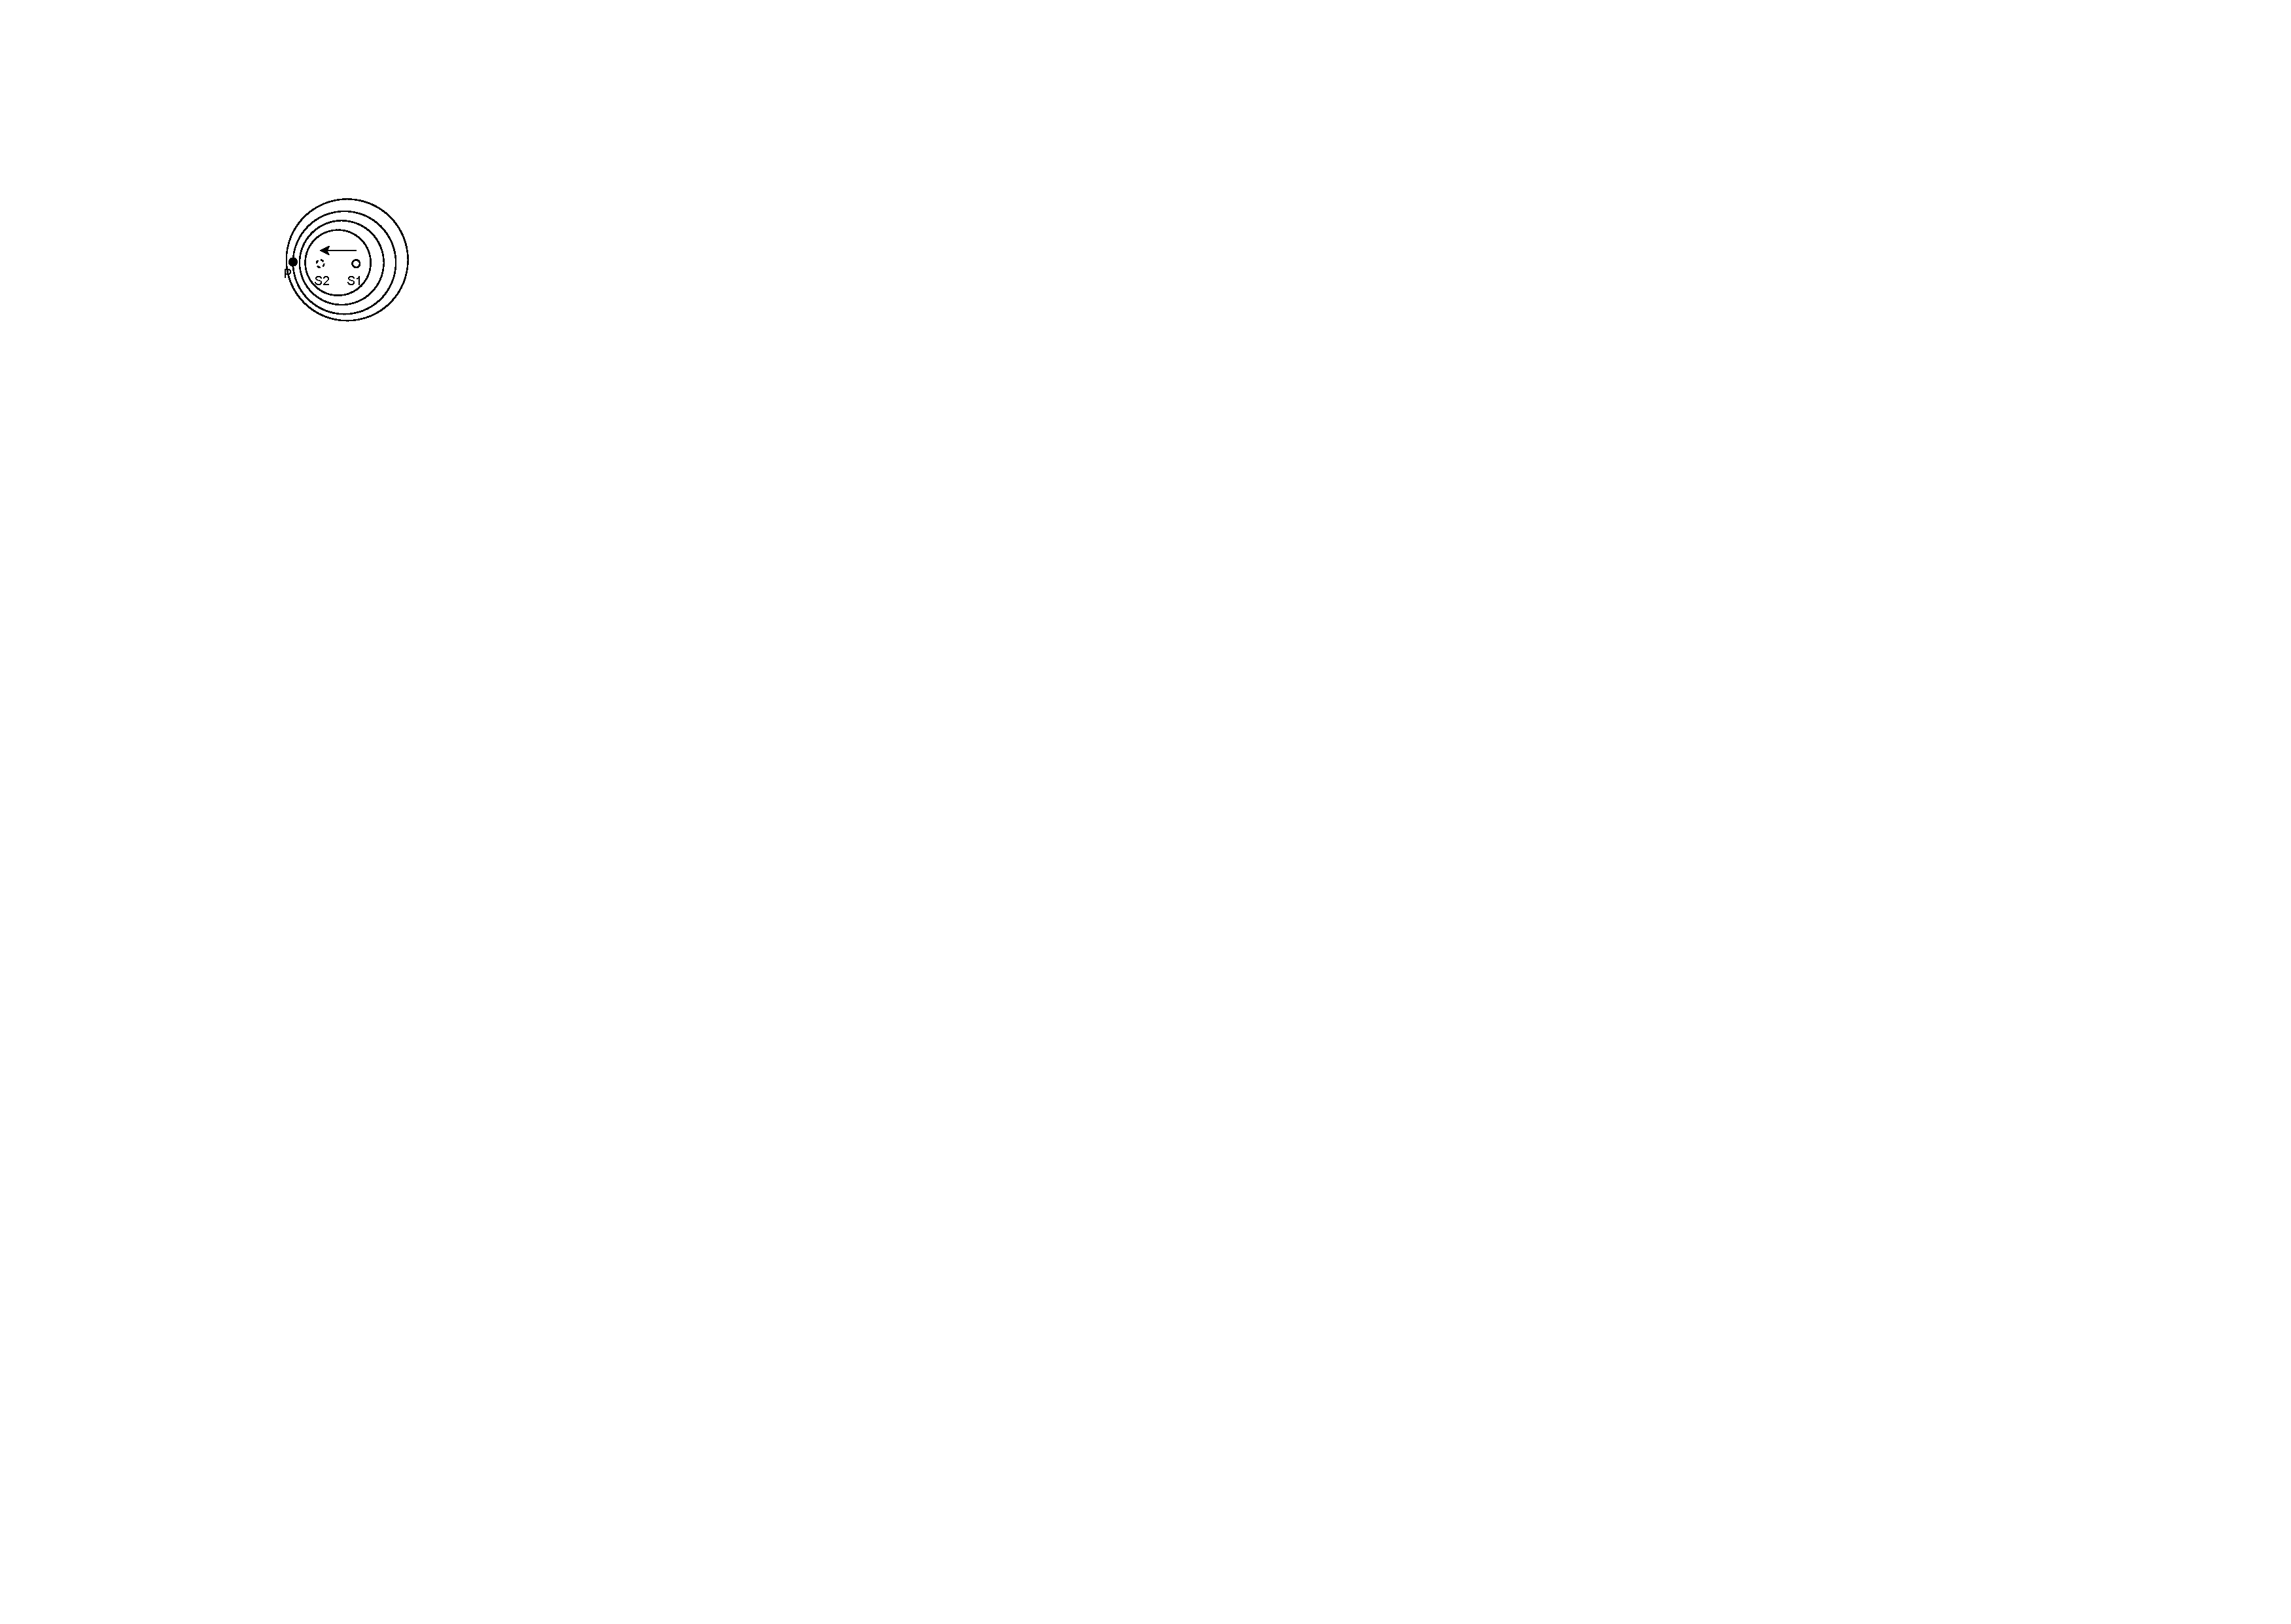
\includegraphics[width=4cm]{fig/2-fig/多普勒频移示意图.drawio.pdf}
    \caption{多普勒频移示意图}
    \label{fig:多普勒频移示意图}
  \end{figure}




由于波源和接收体之间的相对运动而产生的频率变化值的大小与相对运动的速度之间存在定量推导关系,从而使得多普勒频移广泛应用于激光速度/位移测量领域。如图\ref{fig:多普勒频测速示意图}所示,接收体处在\(P\)点,波源从点\(S1\)以速度\(v\)朝着点\(S2\)运动时,有:
\begin{equation}\label{eq:多普勒频测速原理1}
    \Delta L=dcos\theta=v\Delta tcos\theta.
\end{equation}
\begin{figure}[htb]
    \centering
    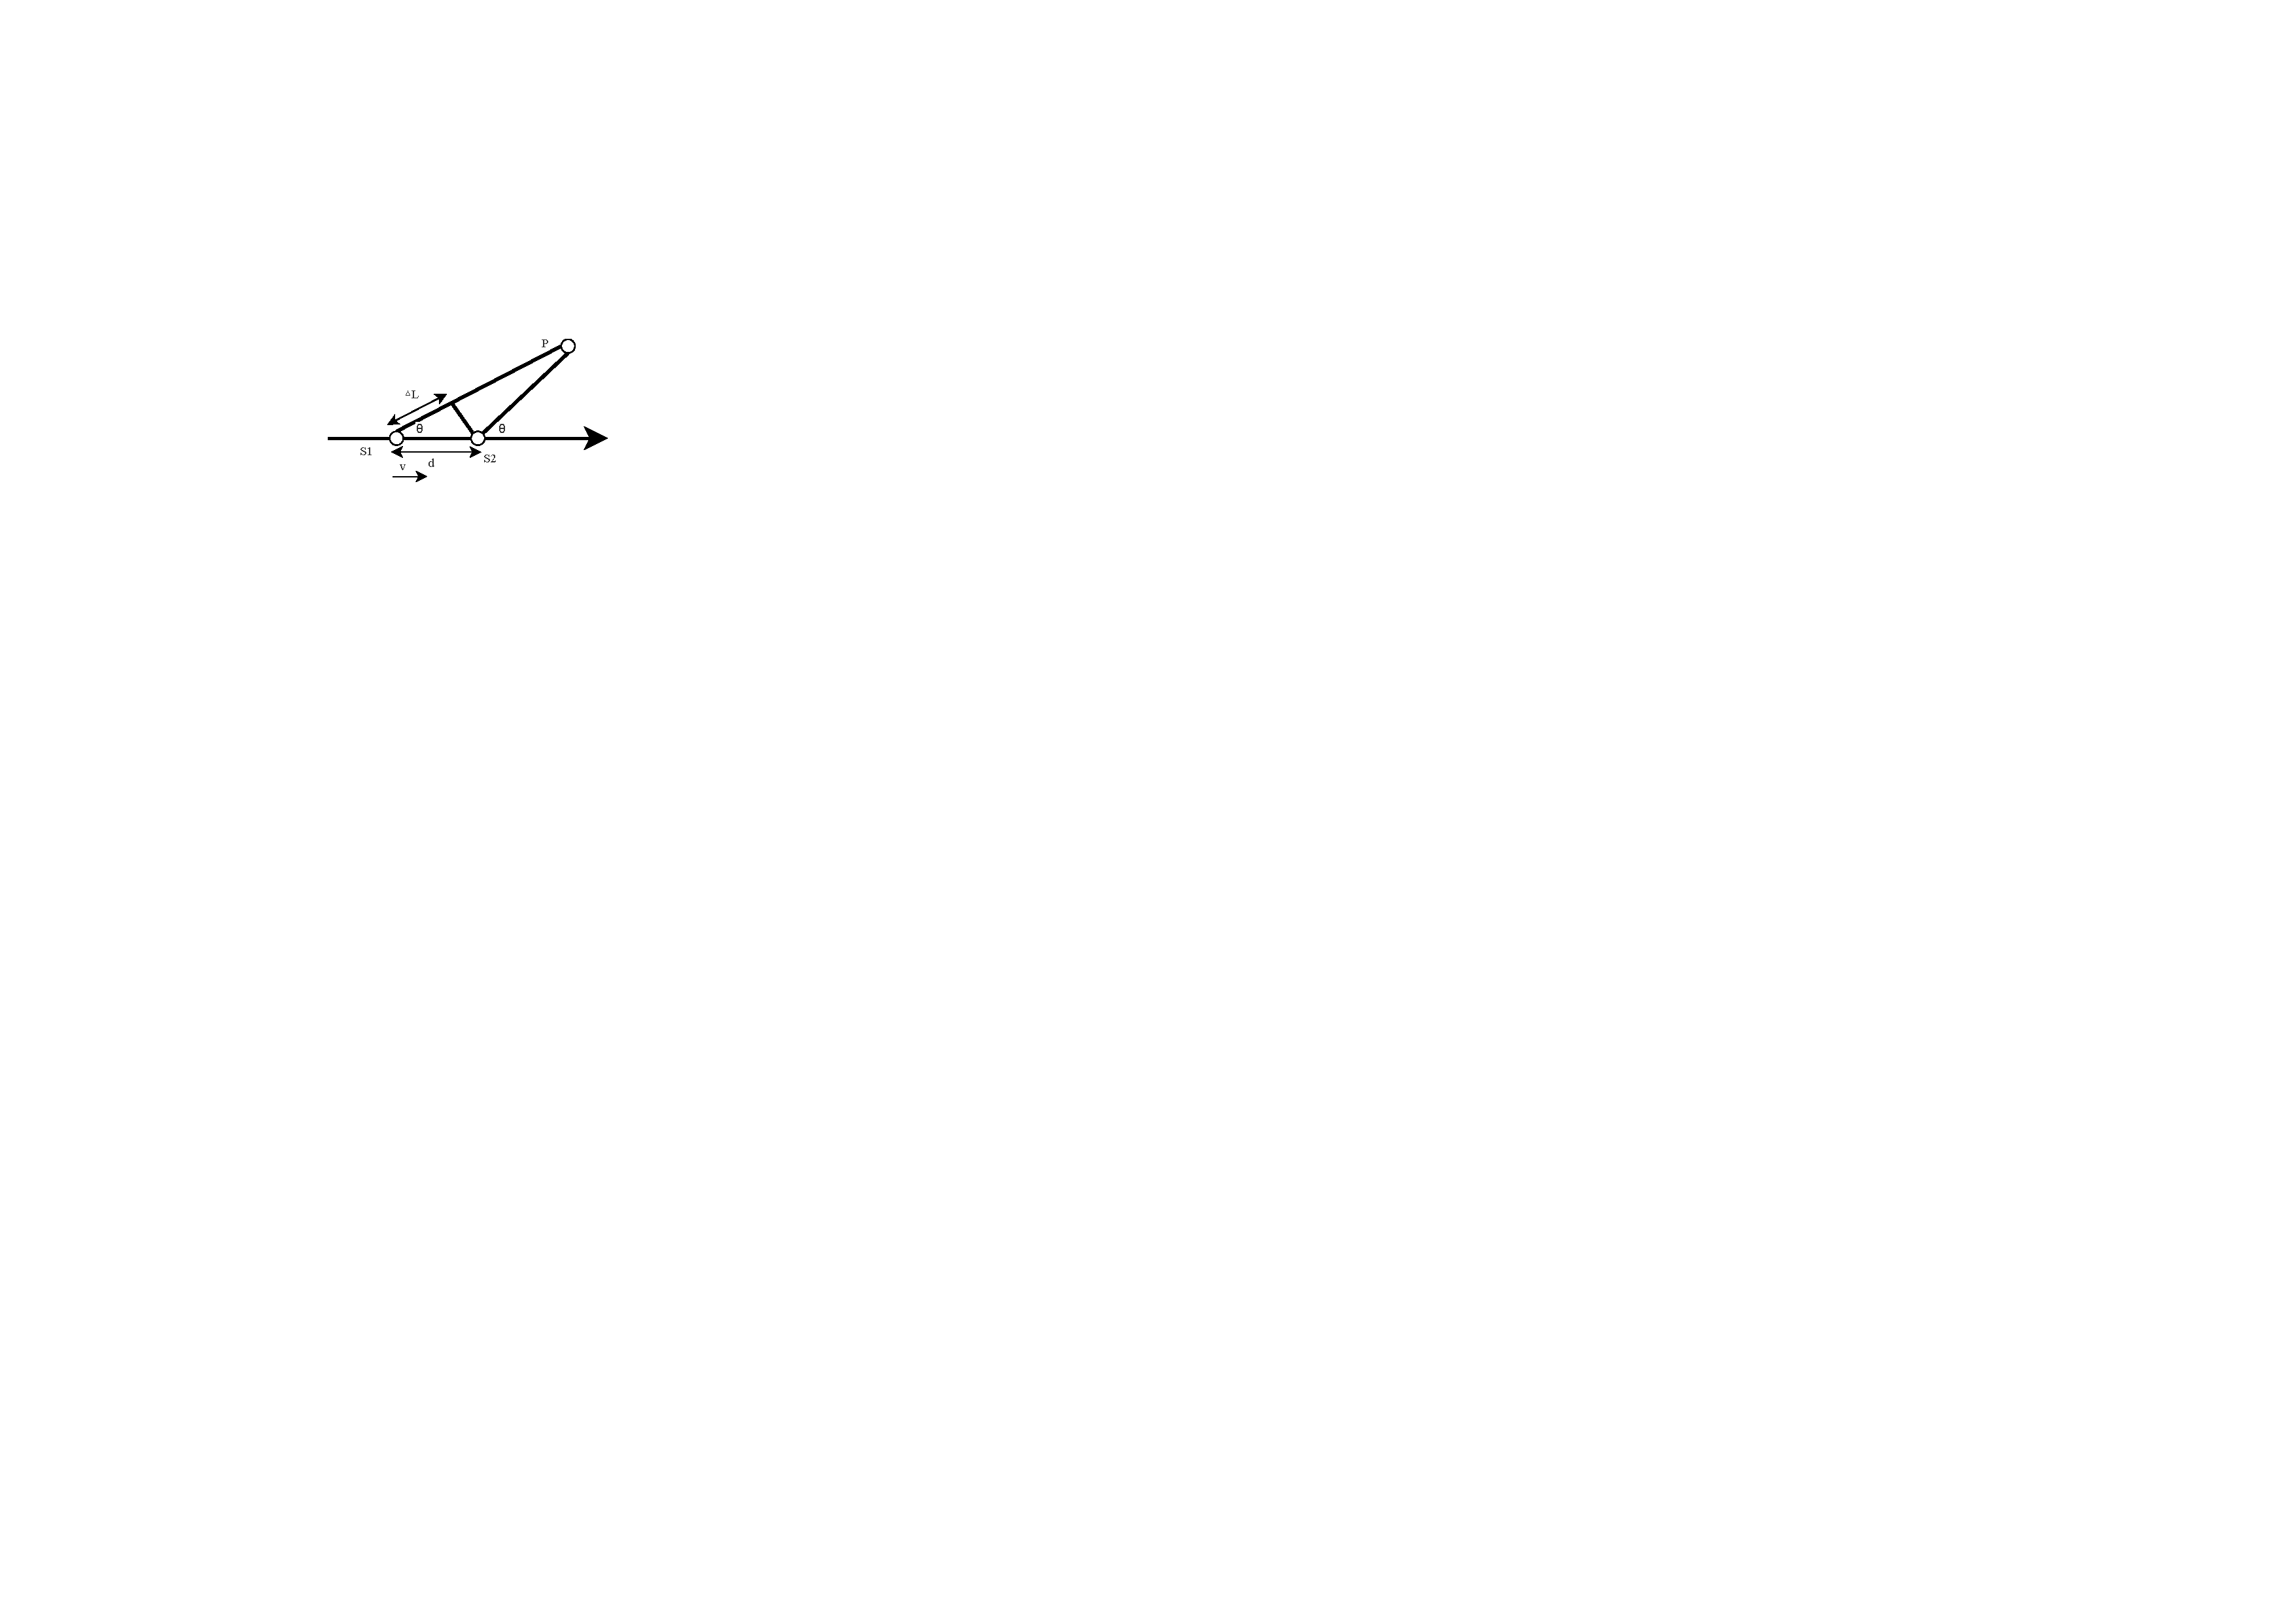
\includegraphics[width=8cm]{fig/2-fig/多普勒频测速示意图.drawio.pdf}
    \caption{多普勒频测速示意图}
    \label{fig:多普勒频测速示意图}
  \end{figure}

式\eqref{eq:多普勒频测速原理1}中\(\theta\)是\(S1\)和\(S2\)处出射波的夹角,\(\Delta L\)两处位置的波程差,\(\Delta t\)为运动所需的时间。由于在实际测量中,波源或者接收体在单位时间内运动距离相比于波源和接收体之间的距离很小,所以可以近似认为\(S1\)和\(S2\)两处的\(\theta\)是相同的\cite{百度百科-多普勒频移},由于波的传播路程差导致的相位变化值为:
\begin{equation}\label{eq:多普勒频测速原理2}
    \varphi=\frac{2\pi \Delta L}{\lambda}=\frac{2\pi v\Delta t}{\lambda}cos\theta.
\end{equation}


对式\eqref{eq:多普勒频测速原理2}左边进行变换,即可得到多普勒频移与运动速度v之间的关系:

\begin{equation}\label{eq:多普勒频测速原理3}
    \varphi_d=\frac{\Delta varphi}{2\pi \Delta t}=\frac{v}{\lambda}cos\theta.
\end{equation}



\subsection{拍频现象}
对于两个振动方向相同、振动频率相同并且相位差恒定的简谐波叠加,会在空间中产生强弱相间的固定分布,这种现象称为干涉。如若两个简谐波的振动频率略有差异,其叠加时会在空间中产生幅值随时间变化的周期性分布,这种现象则称为拍\cite{基于拍频测量温度和旋光角的方法研究},拍频则定义为单位时间内合振幅周期性强弱变化的次数。

假设两个振动方向相同的简谐波的方程为
\begin{equation}\label{eq:简谐波方程1}
    x_1=A_1cos\omega_1t.
\end{equation}
\begin{equation}\label{eq:简谐波方程2}
    x_2=A_2cos\omega_2t.
\end{equation}

上式中\(A_1=A_2\),并且\(|\omega_1-\omega_2|<<\omega_1+\omega2\),那么\(x_1\)和\(x_2\)在空间中相遇叠加产生的拍的方程为:
\begin{equation}\label{eq:简谐波叠加后方程}
   x=x_1+x_2=2Acos(\frac{\omega_2-\omega_1}{2}t)cos(\frac{\omega_2+\omega_1}{2}t).
\end{equation}

\begin{figure}[htb]
    \centering
    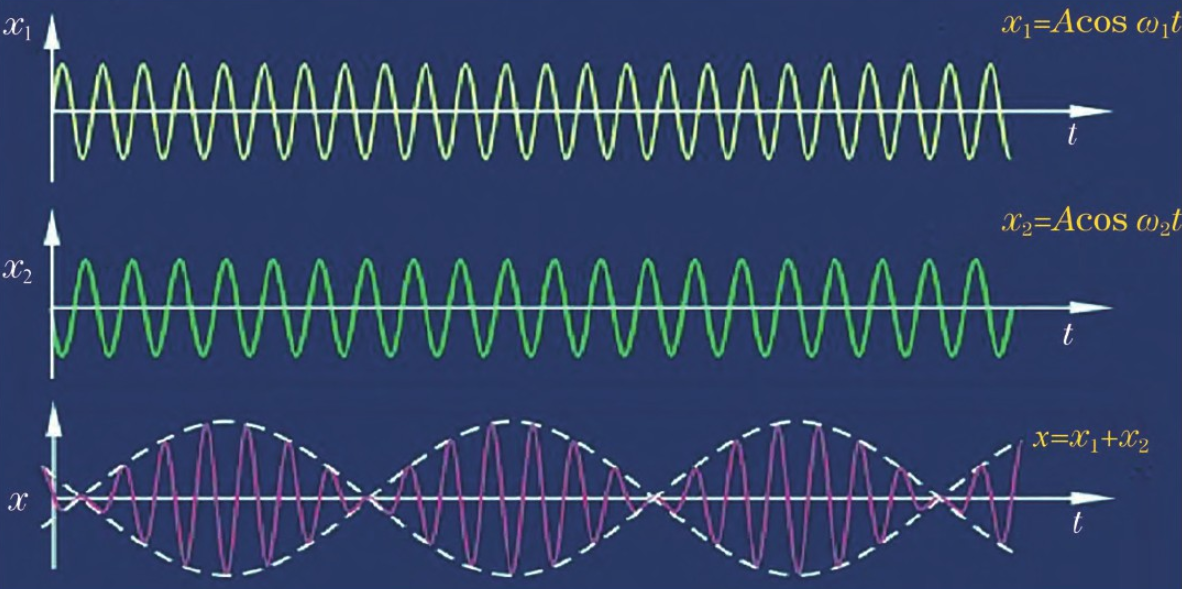
\includegraphics[width=12cm]{fig/2-fig/拍频波形示意图.jpg}
    \caption{拍频波形示意图\cite{激光外差干涉技术在光刻机中的应用}}
    \label{fig:拍频波形示意图}
    \end{figure}
上式中\(|2Acos(\frac{\omega_2-\omega_1}{2}t)|\)为\(x_1\)和\(x_2\)在空间中叠加后拍的幅值,可以看出这是一个随时间周期性变化的值,而\(\frac{\omega_2+\omega_1}{2}\)则为拍的角频率,这也是一个随着时间周期性变化的值,两者共同导致了拍在波形上表现为周期性变化的形式,如图\ref{fig:拍频波形示意图}所示。

并且由式\eqref{eq:简谐波叠加后方程}可以看出,拍的频率为两个简谐波的原始频率之差,虽然当前激光的频率通常很高(约为\(10^{14}Hz\)量级),这使得目前的光电探测器无法响应\cite{激光外差干涉技术在光刻机中的应用},但通过拍频现象,即可将高频的信息转变为低频信息,便于光电探测器响应。



\section{激光干涉仪原理}
\subsection{单频激光干涉仪}
单频激光干涉仪,也可以称为零差干涉仪,具有精度高、稳定可靠, 且相对成本较低等特点\cite{零差干涉仪用于振动校准中关键技术的研究}。其示意图如图\ref{fig:单频激光干涉仪原理图}所示。
\begin{figure}[htb]
    \centering
    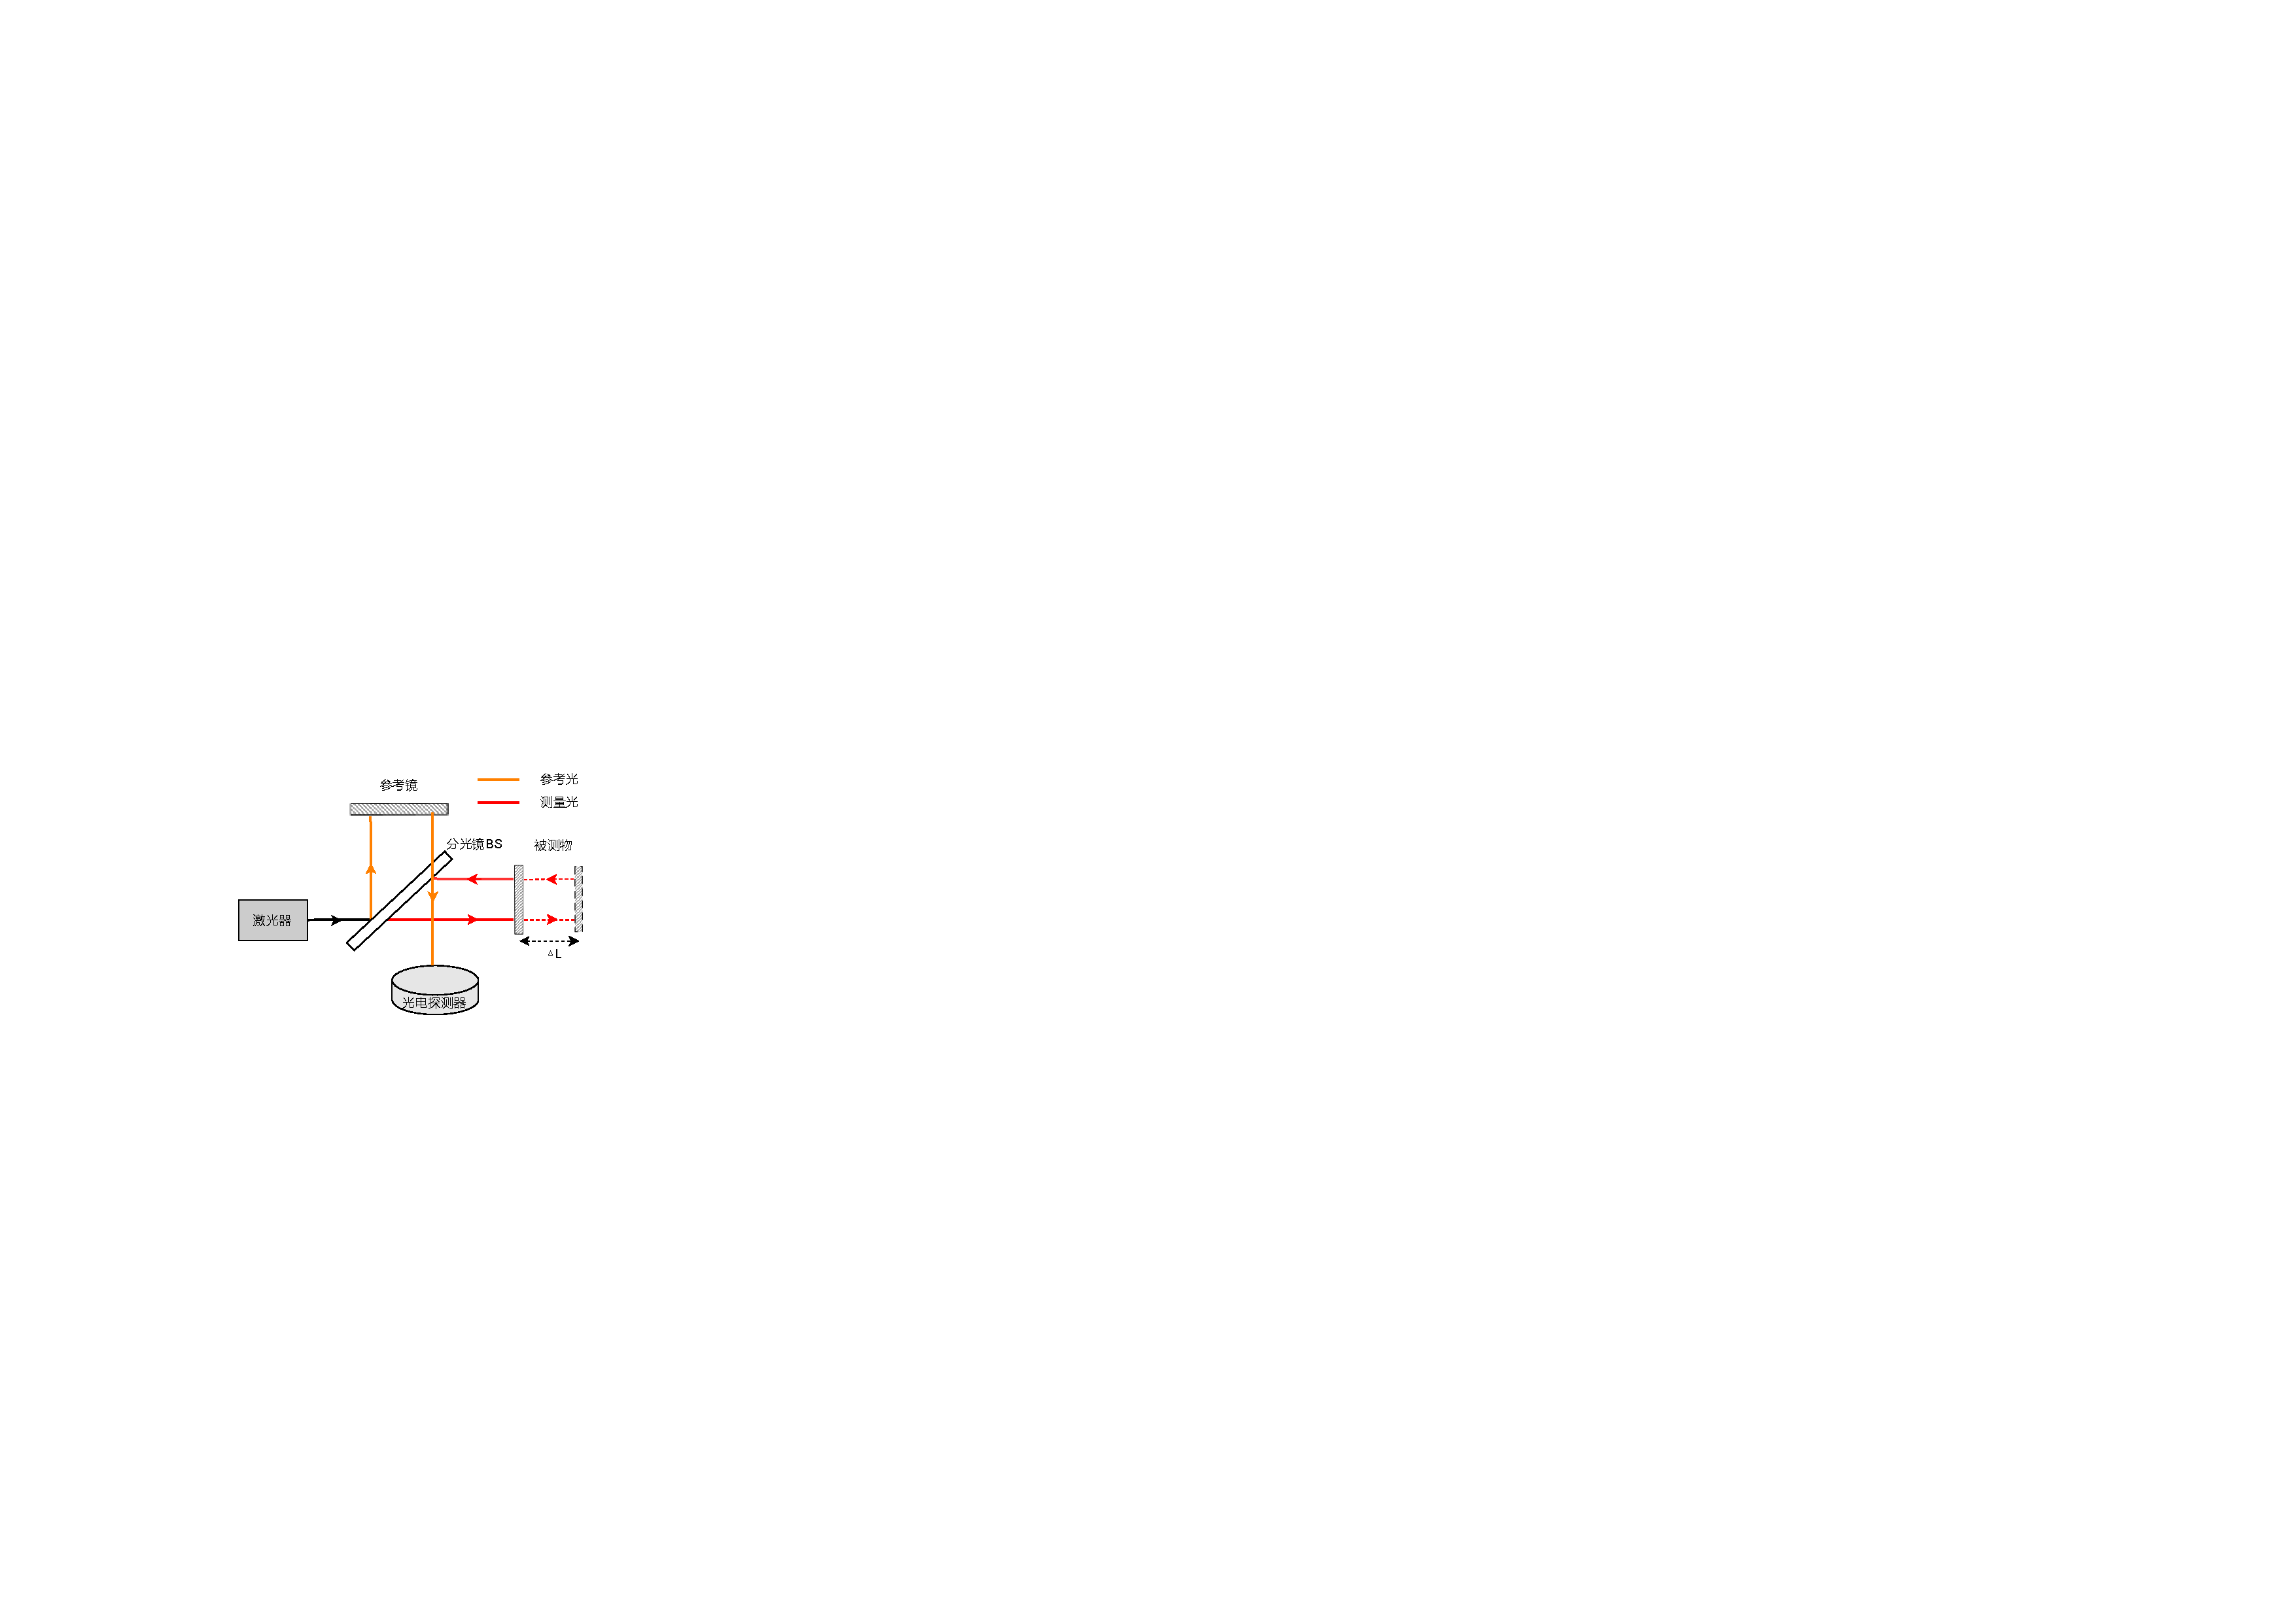
\includegraphics[width=8cm]{fig/2-fig/单频激光干涉仪原理图.drawio.pdf}
    \caption{单频激光干涉仪原理图}
    \label{fig:单频激光干涉仪原理图}
\end{figure}

激光器出射的激光经过分光镜BS后产生两束光:一束进入参考臂,并被参考镜反射,另一束进入测量臂,并被被测物体反射,当被测物体位移为\(\Delta L\)时,测量光会携带上对应的多普勒频移\(f_d\),两束光分别经参考镜和被测物体反射后会再次汇聚,随后射入光电探测器,根据相位的变化即可反推被测物体的位移。

\subsection{双频激光干涉仪}
双频激光干涉仪结构如图\ref{fig:双频激光干涉仪原理图}所示,激光出射的含有\(f_1\)和\(f_2\)两个频率成分的激光经过偏振分光棱镜(polarization beam splitter,PBS)分为测量光\(f_1\)和参考光\(f_2\),测量光\(f_1\)进入测量臂之后,携带上被测物体位移\(\Delta L\)的多普勒频移\(\Delta f\)。由于测量臂和参考臂上各放置了一块四分之一玻片(Quarter Wave Plate,QWB),测量光和参考光在返回PBS之前都经过两次QWB,使得其偏振态发生改变,原本透射的测量光再次返回PBS时变为反射,原本反射的参考光再次返回PBS时变为透射,参考光和测量光汇聚,耦合进光纤,由采集板卡从多普勒频移\(\Delta f\)解调出被测物体的位移\(\Delta L\)。
\begin{figure}[htb]
    \centering
    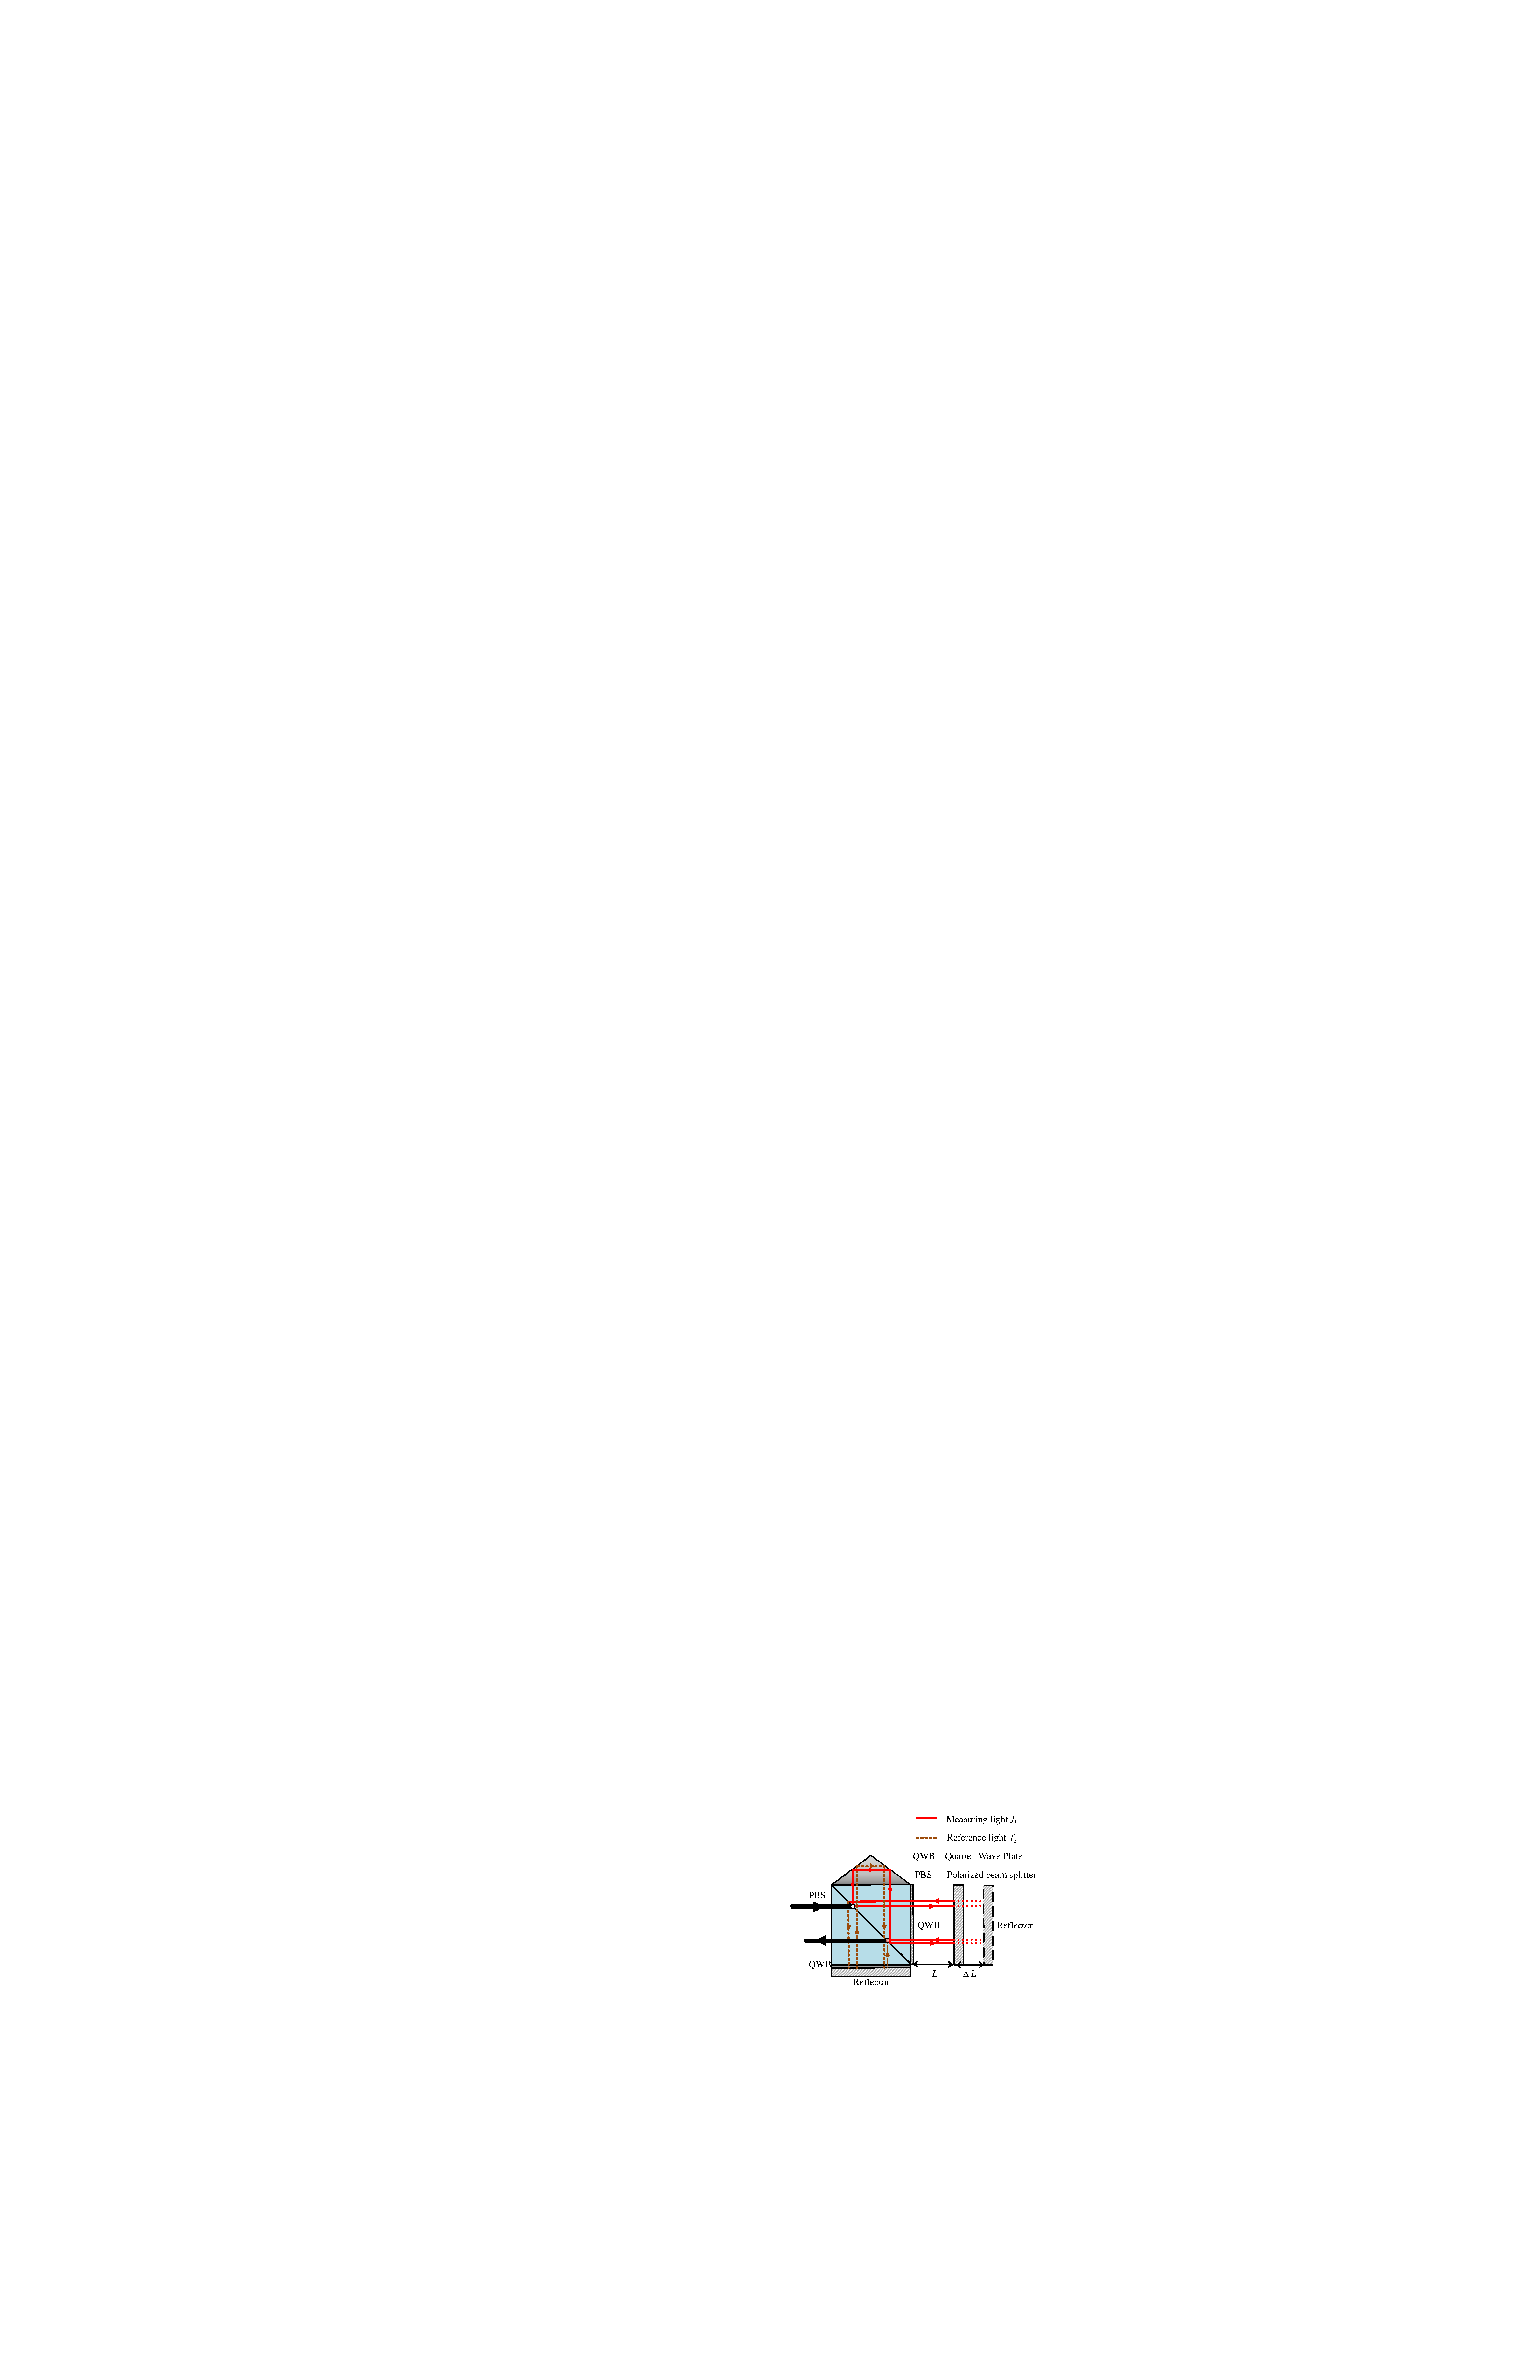
\includegraphics[width=9cm]{fig/2-fig/双频激光干涉仪原理图.pdf}
    \caption{双频激光干涉仪原理图}
    \label{fig:双频激光干涉仪原理图}
\end{figure}

\section{双频激光干涉仪的环境误差及其成因}
在真实的测量场景中,双频激光干涉仪的测量值\(D\)是指干涉仪系统实际输出的位移值。是由条纹数\(N\)乘上干涉仪系统的分辨率\(R_{es}\)得到的,而条纹数\(N\)与光程的变化有光,即:
\begin{equation}\label{eq:测量值与光程的关系}
    D=R_{es}{\times}N=R_{es}{\times}\frac{\Delta L{\times}n_0{\times}M_o}{\lambda{\div}M_e}=\Delta L{\times}n_0.
\end{equation}

式\eqref{eq:测量值与光程的关系}中,\(n_0\)为真空中的空气折射率,近似可认为1,干涉仪的分辨率\(R_{es}\)与激光的实际波长\(\lambda\)、电子细分\(M_e\)和光学细分\(M_o\)有关。电子细分\(M_e\)由干涉仪系统的采集板卡决定,常见的有32、64、128、256......2048等,而光学细分\(M_o\)只与干涉仪的设计结构有关,对于采用角锥镜为被测对象的干涉仪,光学细分一般为2,采用平面镜为被测对象的干涉仪,光学细分一般为4,干涉仪的分辨率具体计算公式如下:
\begin{equation}\label{eq:分辨率与细分的关系}
    R_{es}=\frac{\lambda}{M_o{\times}M_e}.
\end{equation}

电子细分和光学细分在测量过程中一般不会引入太大的误差,但是激光的波长跟测量环境中的空气折射率有关,而外界环境因素(温度、气压等)的变化也会导致空气折射率变化\(\Delta n\),此时,干涉仪系统测量值\(D\)不仅包括被测物体的位移\(\Delta L\),还包括由于折射率变化引起的光程变化\(\Delta l\),即:
\begin{equation}\label{eq:实际的位移公式}
    D=\Delta L(\Delta n+n_0)+L\Delta n.
\end{equation}

但由于测量臂长度\(L\)一般远大于被测物体位移\(\Delta L\),由式\eqref{eq:测量值与光程的关系}和式\eqref{eq:实际的位移公式}可得,由于外界环境因素(温度、气压等)引起的误差为:
\begin{equation}\label{eq:环境误差公式}
    D=[\Delta L(\Delta n+n_0)+L\Delta n]-\Delta Ln_0=\Delta n(\Delta L+l) \approx \Delta n \Delta L.
\end{equation}

根据相关文献的描述\cite{徐建2013双频激光干涉仪系统线性测量误差主要来源及减小误差的方法分析},在对上述环境因素不进行任何控制或补偿的情况,空气折射率的变化可能会达到50ppm,如果仅对测量环境温度进行控制,其余因素的变化也可能导致空气折射率变化20ppm以上。放在双频激光干涉仪领域,根据式\eqref{eq:环境误差公式}可知,空气折射率变化需要乘上测量臂长度才是双频激光干涉仪的环境误差,这就导致当测量臂长度较小时,这部分的误差是可以忽略不计的,但随着测量臂长度的增加,双频激光干涉仪的环境误差也随着增大。以10mm的测量臂长度为例,当温度变化超过\(0.1\)$^{\circ}$C时,这部分的误差就可能已经超过1nm了,所以需要对上述的环境误差进行补偿。

\section{基于Edlen公式的补偿方法及其局限性}
\subsection{Edlen公式补偿方法}
1965年,Edlén基于洛伦兹方程和空气密度方程推导出了空气密度因子,并基于空气密度因子提出Edlen公式用于空气折射率的修正\cite{2015Refractive}。最近一次广泛承认的修正是Boensch等\cite{1998Fit}于1998年优化的Edlen公式,其中关于空气折射率与温度和气压的关系如式\eqref{eq:原始Edlen公式}所示。
    \begin{equation}\label{eq:原始Edlen公式}
    (n\,-\,1)_{tp}=\frac{Pn_0}{93214.60}\frac{[1\,+\,10^{-8}(0.5953\,-\,0.009876T)]}{1\,+\,0.0036610T}.
    \end{equation}

式\eqref{eq:原始Edlen公式}中 \((n-1)_{tp}\)为考虑温度与气压时的空气折射率,\(n_0\)为理想情况下空气折射率,\(P\)为环境气压,\(T\)为环境温度。当气压\(P\)取一个标准大气压(101.325\(kPa\)),温度\(T\)从\(20\)$^{\circ}$C变化到\(30\)$^{\circ}$C时,折射率随温度的变化如图\ref{fig:折射率-温度}所示;当温度\(T\)取\(20\)$^{\circ}$C,而气压\(P\)在一个标准大气压附近变化时,折射率随着气压的变化如图\ref{fig:折射率-气压}所示。
\begin{figure}[htb]
    \centering
    \subfigure[折射率随温度变化]{
      \begin{minipage}[b]{0.70\textwidth}
        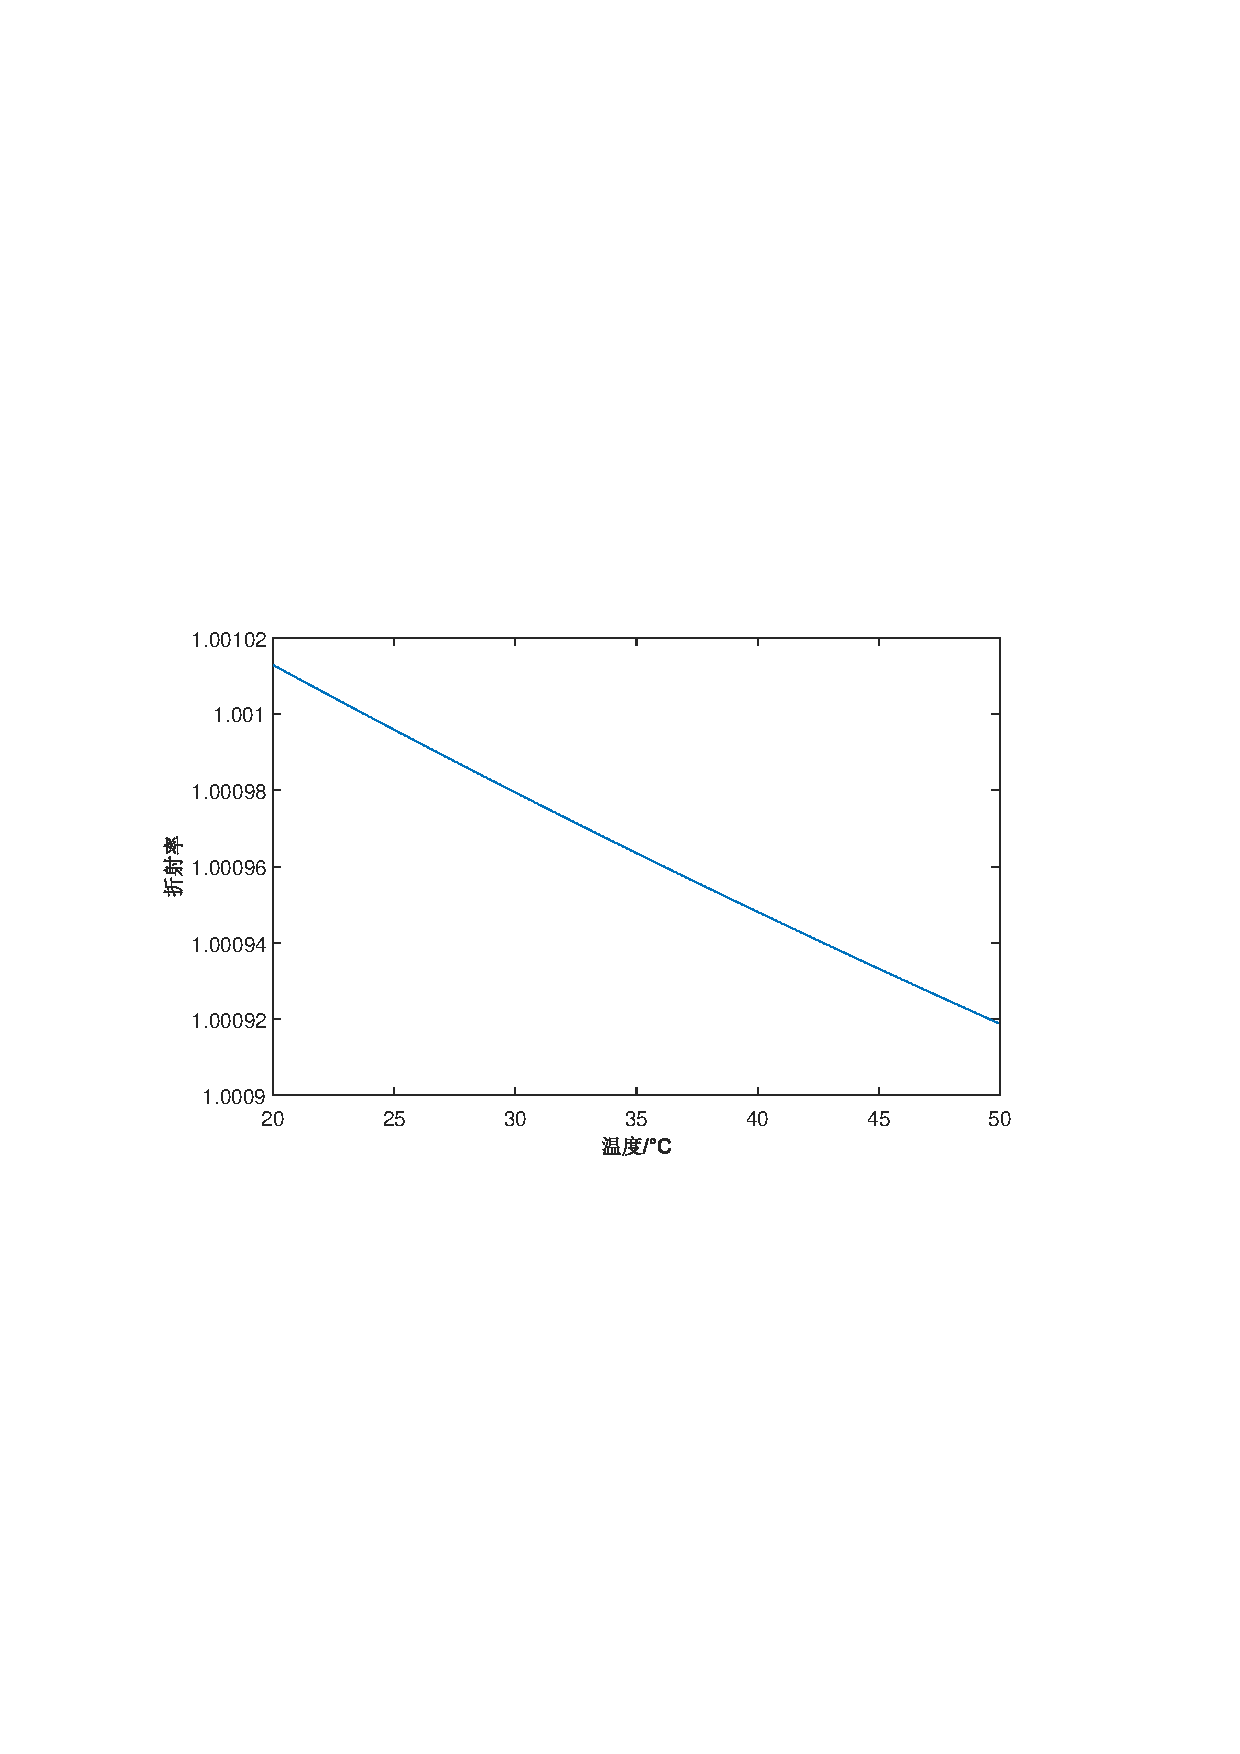
\includegraphics[width=10cm,height=5cm]{fig/2-fig/折射率随温度变化.pdf}
      \end{minipage}
      \label{fig:折射率-温度}
    }
    \subfigure[折射率随气压变化]{
      \begin{minipage}[b]{0.70\textwidth}
        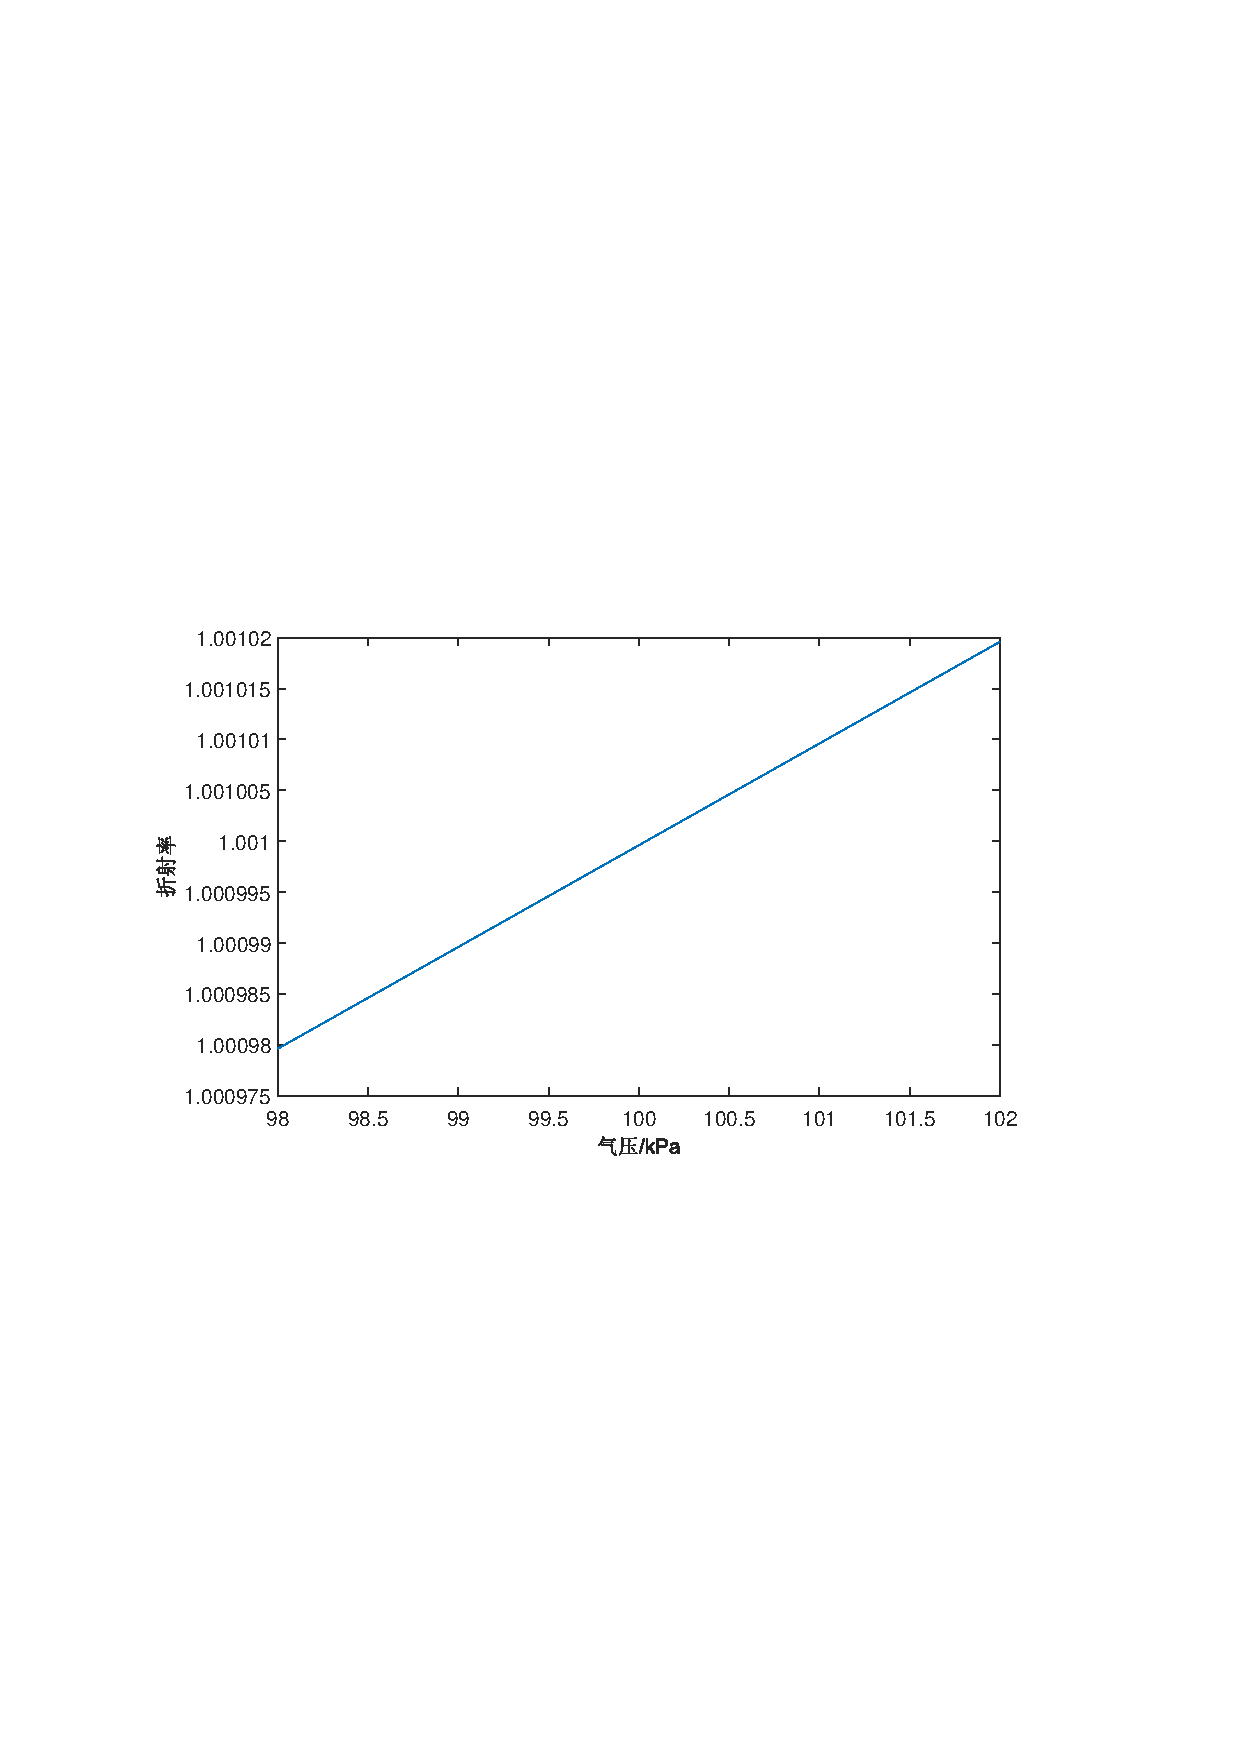
\includegraphics[width=10cm,height=5cm]{fig/2-fig/折射率随气压变化.pdf}
      \end{minipage}
      \label{fig:折射率-气压}
    }
    \caption{折射率变化图}
    \label{fig:折射率变化图}
  \end{figure}

可以看出,在上述范围内,空气折射率和温度/气压变化呈近似线性\cite{李博2021温度对激光干涉法测量气体动态压力的影响}。对式\eqref{eq:原始Edlen公式}中各因子求偏导数,可以得到空气折射率变化\(10^{-8}\)时温度和气压的变化因子分别为\(3.73Pa\)和\(0.01\)$^{\circ}$C\cite{2015Approach}。通过仿真分析,可得出温度和气压对空气折射率的影响呈线性或近线性关系,\eqref{eq:原始Edlen公式}可简化如下\cite{elden公式法在双频激光干涉仪测量系统的应用}:
\begin{equation}\label{eq:线性形式的Edlen公式}
    \Delta n=\frac{\partial n}{\partial T}\,\Delta T+\frac{\partial n}{\partial P}\,\Delta P
    =-9.36*10^{-7}\Delta T\,+\,2.68*10^{-9}\Delta P.
    \end{equation}

式\eqref{eq:线性形式的Edlen公式}中\(\Delta n\)为空气折射率的变化值,\(\Delta T\)为温度变化值,单位为$^{\circ}$C,\(\Delta P\)为气压变化值,单位为\(Pa\)。由温度传感器和压力传感器测量出对应的温度值和压力值,带入式\eqref{eq:线性形式的Edlen公式}计算出空气折射率变化值,再由式\eqref{eq:环境误差公式}即可求出干涉仪的环境误差。
\subsection{局限性}
现有的Edlen公式用于干涉仪环境补偿有着如下局限性:
\begin{enumerate}
  \item 波长不匹配:现有的Edlen公式是根据644.0nm、508.7nm、480.1nm和467.9nm四个波长段的测量数据得出的,而干涉仪由于对光束横模模式和频率稳定性的高要求,所用的激光光源多为波长段为633nm的氦氖激光器,两者在波长段上并不匹配。
  \item 温度不匹配:现有的Edlen公式的适用温度位标准条件下温度20$^{\circ}$C\cite{2020Effect},而干涉仪广泛使用于光刻机中或其它超精密测量领域,其工作环境温度大多为22$^{\circ}$C或常温范围(24$^{\circ}$C-26$^{\circ}$C)。
  \item 主观性强:有的Edlen公式是根据实验数据人为总结的,带有很大的主观性。
\end{enumerate}


\section{本章小结}
本章主要介绍了激光位移测量的基本理论和干涉仪环境误差的成因及Edlen公式补偿方法。首先阐述了激光位移测量领域广泛利用的两个原理:多普勒频移和拍频。随后介绍了单频激光干涉仪和双频激光干涉仪结构和光路,并从双频激光干涉仪一些参数值说起,其中包括分辨率、电子细分、光学细分等,详细分析了环境误差的成因以及影响大小。最后介绍了目前广泛应用于双频激光干涉仪环境误差补偿的Edlen公式,并说明当前Edlen公式存在着波长不匹配、温度不匹配、主观性强三个局限性,为后文的工作提供了基础。